\chapter{Comparison of Gene Network Inferred by RNA-Seq analysis}
\section{Introduction}

Differential expression (DE) and pathway analysis are widely used
techniques to identify candidate genes and pathways associated with
phenotypes or diseases~\cite{smith2011systems,beane2011characterizing,
  li2012rna}.  The advent of high-throughput technologies such as
microarrays and next-generation sequencing (NGS) has led to an
explosion of tools and pipelines for exploring expression data.  Most
of the tools for DE and pathway analyses rely on publically
available gene sets such as Ensembl for quantification of gene
expression and downstream pathway annotation.

% @CTB maybe move, maybe keep, not sure yet :)
%Ensembl gene models are maintained and updated by the Ensembl project
%(\texttt{http://ensembl.org}), which provide gene annotations for 70
%species~\cite{flicek2013ensembl}.  The annotations are linked to
%external information such as gene names from HUGO Gene Nomenclature
%Committee (HGNC), the Protein Databank (PDB), the Universal Protein
%Resources (UNIPROT), the RefSeq collection of Reference Sequences, and
%the UCSC Genome Browser. These annotations include evidence taken from
%tissue-specific RNA-Seq data.  This provides a great resource for
%studying tissue-specific gene expressions as well as alternate splice
%forms.  KEGG pathway is a reference knowledge base that provides
%information for understanding higher-level functions of cellular
%processes and organism behaviors; it is maintained at
%\texttt{http://www.genome.jp/kegg}. These publically available
%information resources have been extremely useful for biologists in the
%genomic era, especially those who study model organisms such as human
%and mouse.

Recently, RNA sequencing (RNA-Seq) by NGS technology has not
only allowed biologists to study expression of annotated
genes but also to discover novel genes and isoforms as well
as to obtain evidence of transcribed but untranslated
regions~\cite{pickrell2010understanding,
lu2010function,otto2010new,raghavachari2012systematic}.
This technology also provides an opportunity for biologists
to generate more comprehensive transcriptomes for organisms
by reconstructing transcript sequences from short reads
using \textit{de novo} assembly or \textit{ab initio}
methods.  However, because executing these tools requires
significant computational expertise, researchers may rely on
existing annotation resources instead of building new gene
models.

The consequences of using different gene models on gene
expression analysis and pathway predictions have not been
explored.  We speculated that more comprehensive gene models
could affect these analyses significantly, especially in
organisms where the available gene annotations are
relatively sparse compared to NIH model organisms.
Incomplete gene models are insensitive to read mapping,
which would affect predicted gene expression levels and the
significance of differential expression calculations; in
addition, missing splice variants and exons limit the power
of differential isoform expression analysis.  Missing gene
models also decrease the power of GO and KEGG pathway
analyses by potentially eliminating genes important for
pathways.

In this article, we present comparisons of differential
expression computations and KEGG pathway analyses of RNA-seq
data between Ensembl gene models, {\em ab initio} and {\em
de novo} constructed gene models, and merged gene models
built from all of the above.  We also show the effect on
predictions of differentially expressed pathways when
including KEGG pathway annotations from human in our
analysis.  We demonstrate that the gene models used and the
extent of the annotation source significantly affect
predictions and their statistical support.  Finally, we
discuss the implications for the investigation of organisms
with relatively incomplete gene annotations.

% Results and Discussion can be combined.
\section{Results}

\subsection{The set of differentially expressed genes varies widely
by gene model set used}

% @CTB: side note, make sure we discuss ``why rsem?'' and ``are our results
% general beyond RSEM?'' down below, in dsicussion

The first step in pathway enrichment analysis is to identify
differentially expressed genes.  Starting with each of four
different sets of gene models, we used RSEM to estimate gene
expression and then applied EBSeq to identify differentially
expressed genes.  For gene models, we used the public
Ensembl gene models together with three sets of custom gene
models.  The custom-constructed gene models were, (1)
constructed by {\em de novo} mRNAseq assembly with
Velvet/Oases~\cite{Zerbino:2008vu,Schulz:2012je}, (2) a
genome reference-guided gene set constructed with
Cufflinks~\cite{Trapnell:2010kd}, and (3) a merged gene set
constructed with Gimme from a combination of all three other
gene sets; see Methods for details.  All custom gene sets
were constructed using the same Marek's Disease Virus
mRNAseq data sets used for differential expression analysis.

We next examined the rate of read mapping to the gene
models.  The percentages of reads mapped to the Ensembl
models are lowest in all samples compared to other gene
model sets (Table ~\ref{tab:mapped-reads}).  Fewer than 60\%
of reads mapped to the Ensembl models indicating that the
gene models do not include all coding and non-coding regions
expressed in the samples.  The results from the assembly
models confirm that many reads are from regions not included
in the Ensembl models. Note that the number of mapped
single-end reads is highest in the assembly models, even
though those models have the fewest distinct genes.

\begin{table}[!ht]
\caption{
\textbf{Rate of reads mapped to Ensembl-matched gene models}
}
\begin{center}
\begin{tabular}{ccccccc}
\hline
& Single & & Paired-end & & Total & \\
& Control & Infected & Control & Infected & Genes \\
\hline
Ensembl & 61.93\% & 63.59\% & 57.83\% & 59.24\% & 15,943 \\
Assembly & 81.40\% & 84.01\% & 64.24\% & 66.75\% & 9,002 \\
Cufflinks & 78.16\% & 81.28\% & 76.56\% & 77.44\% & 14,020 \\
Merged & 78.14\% & 81.48\% & 75.87\% & 77.23\% & 13,973 \\
Total reads & 27,618,789 & 29,693,654 & 42,632,733 & 30,804,398 & \\
\hline
\end{tabular}
\end{center}
%\begin{flushleft}
%    (-) down-regulated, (+) up-regulated
%\end{flushleft}
\label{tab:mapped-reads}
\end{table}
% However, the number of mapped
%paired-end reads are more reliable due to stringency of paired-end
%mapping criteria.
% @CTB: Likit, were the paired-end reads used to construct the
% gene models?
% @Likit: Yes.

We compared differentially expressed gene predictions
between data sets by linking each gene to an Ensembl gene
via BLAST, which provided a common reference identifier.  A
summary of the correspondence is in
Table~\ref{tab:ensbl_matched}.  From {\em de novo} assembly,
9002 (56.46\%) of the gene models matched to one of the
approximately 16,000 Ensembl genes.  Cufflinks and merged
models matched considerably more of the Ensembl genes --
14020 (87.9\%) and 13973 (87.6\%), respectively.

\begin{table}[!ht]
\caption{
\textbf{Genes and DE genes matched Ensembl genes}}
\begin{center}
\begin{tabular}{ccccc}
\hline
& Ensembl & Assembly & Cufflinks & Merged \\
\hline
All & 15943 & 9002 & 14020 & 13973 \\
DE & 2538 & 2109 & 3433 & 3402 \\
\hline
\end{tabular}
\end{center}
%\begin{flushleft}
%    (-) down-regulated, (+) up-regulated
%\end{flushleft}
\label{tab:ensbl_matched}
\end{table}

Of the genes in the different data sets with identifiable
correspondence to Ensembl, RSEM predicted that between 2109
and 3433 genes were differentially expressed (DE) across the
gene model sets.  However, the number of DE genes shared
between two different gene sets was much lower, with a
maximum of 3069 out of 3428 (89.5\%) DE genes shared between
Gimme and Cufflinks (Figure~\ref{degenes_venn}D).  Gimme
incorporates the Cufflinks gene models, however, and so the
best agreement on DE genes between two independent data sets
is between Ensembl and Cufflinks, where 1991 genes are DE in
both Ensembl (1991 of 2538 DE genes, 78.4\%) and Cufflinks
(1991 of 3428, 58.0\%).  Despite this correspondence, the
number of disjoint DE genes between samples is often equal
to or larger than the number of DE genes in common between
any two gene sets.

\begin{figure}[!ht]
    \begin{center}
        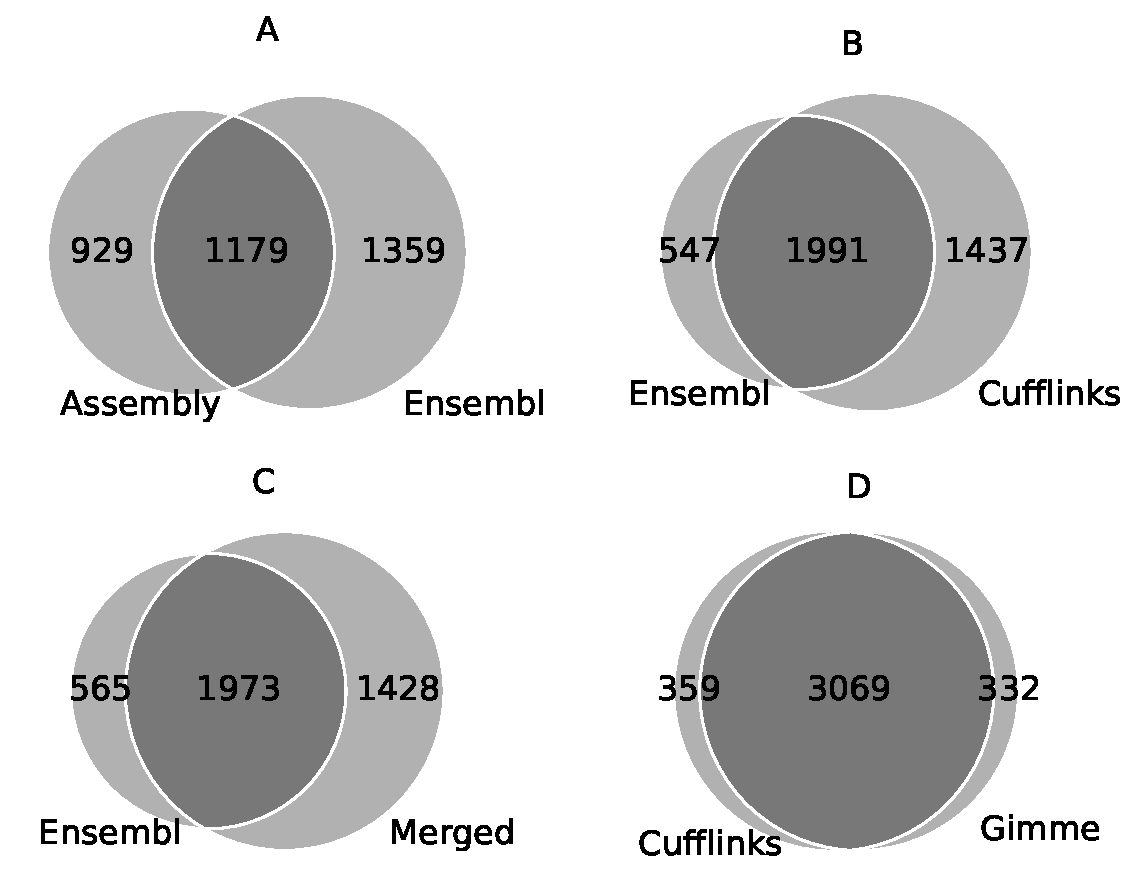
\includegraphics[width=6in]{ensbl-assm-cuff-comb-degenes-venn.pdf}
    \end{center}
    \caption{
        \textbf{Comparison of differentially expressed genes.}
        DE genes were matched to Ensembl genes via BLAST. (A-C) The number of DE
        genes in other gene model sets differ greatly when compared to Ensembl
        models.  (D) Although Cufflinks models were incorporated into Gimme
        models, not all DE genes in Cufflinks were found in Gimme models.
    }
    \label{degenes_venn}
\end{figure}
% @CTB can you do a venn diagram as in Eli's paper for this, do you think?
% @LP I will look at it.

\subsection{Variation in differential expression predictions is due to
variation in read mapping}

To identify the factors contributing to variation in DE
analysis, we examined estimated read counts of genes
identified as differentially expressed in one gene model set
versus another.  For example, the {\em IFNB} gene was not DE
when the Ensembl models were used, but was DE when the
merged Gimme models were used; upon examination, we found
that the number of reads mapping to the {\em IFNB} gene
model was much higher in the merged models
(Figure~\ref{ifnb_count}).  This discrepancy in mapped reads
was due to a substantial number of reads mapped to the
extended regions in the Gimme model, which are not included
in the Ensembl model (Figure~\ref{ifnb}).  Another example
is the {\em IDH3A} gene, shown in Figure~\ref{idh3a}. This
gene was expressed in both control and infected groups, but
is only identified as DE when the Gimme models are used
(Figure~\ref{idh3a_count}).  This is because the complete
$5\prime$ UTR is included in only one of the two Ensembl
isoforms and not in the RefSeq model, whereas both $3\prime$
and $5\prime$ UTRs are included in the Gimme model.  The
size of the $3\prime$ UTR in the Gimme model is slightly
larger than that of RefSeq and the size of the Gimme
$5\prime$ UTR is the same as that of Ensembl model.

\begin{figure}[!ht]
    \begin{center}
        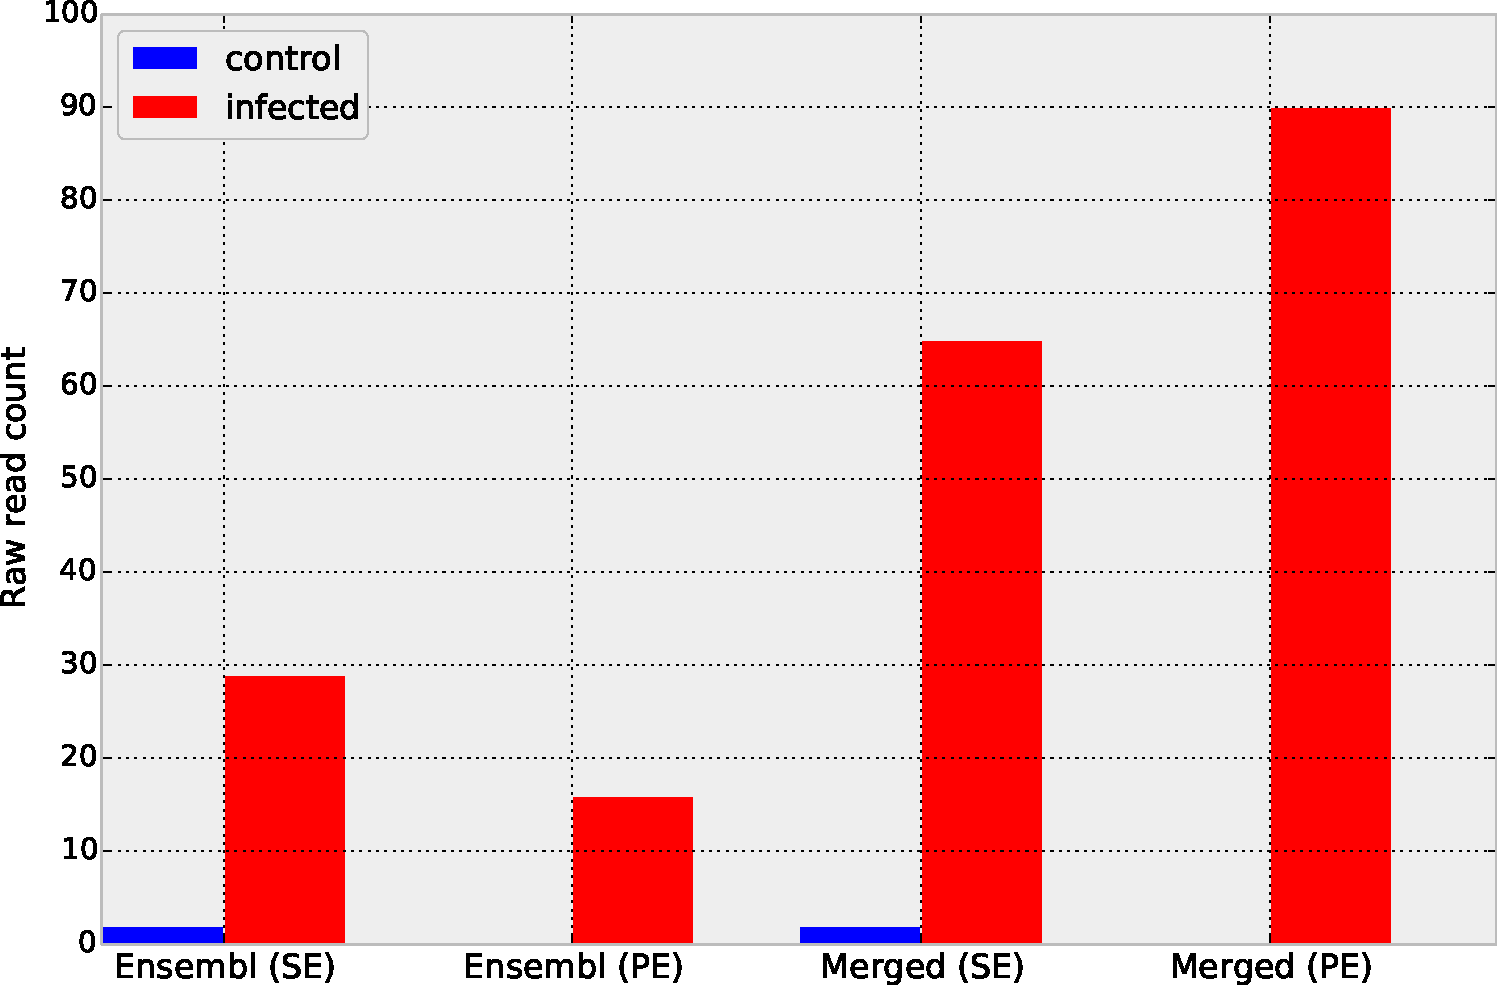
\includegraphics[width=6in]{ifnb-raw-reads-bar.pdf}
    \end{center}
    \caption{
        \textbf{Read counts of {\em IFNB} gene.} SE=single-end, PE=paired-end
    }
    \label{ifnb_count}
\end{figure}

\clearpage\pagestyle{lscape}
\begin{landscape}
\begin{figure}[!ht]
    \begin{center}
        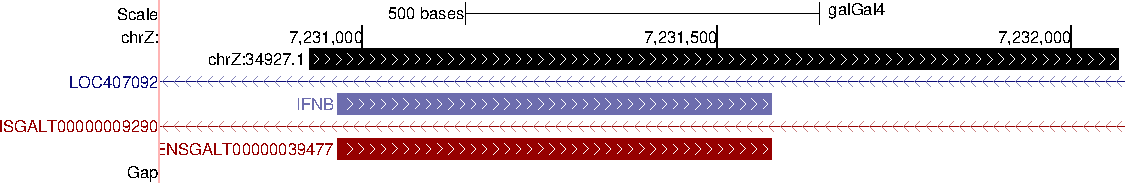
\includegraphics[width=8in]{ifnb.pdf}
    \end{center}
    \caption{
        \textbf{{\em IFNB} gene models from Ensembl
        (ENSGALT00000039477, red), Gimme (chrZ:34927.1, black)
        and RefSeq (blue).}
        RefSeq and Ensembl models only include the CDS region;
        whereas, Gimme model include extended regions that could
        be unstranslated regions (UTRs). The extended regions are
        of notable sizes, which could account for a substantial
        number of mapped reads.
    }
    \label{ifnb}
\end{figure}

\begin{figure}[!ht]
    \begin{center}
        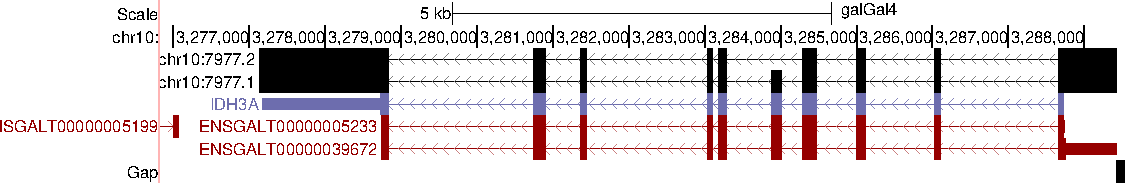
\includegraphics[width=8in]{idh3a.pdf}
    \end{center}
    \caption{
        \textbf{{\em IDH3A} gene models from Ensembl
        (ENSGALT00000005233,39672, red), Gimme
        (chr10:7977.1, chr10:7977.2, black) and RefSeq (blue).}
        RefSeq model only includes CDS and $3\prime$ UTR. Ensembl
        model only includes CDS and $5\prime$ UTR in one isoform.
        Gimme model includes CDS and both UTRs.
    }
    \label{idh3a}
\end{figure}
\end{landscape}
\pagestyle{plain}

\begin{figure}[!ht]
    \begin{center}
        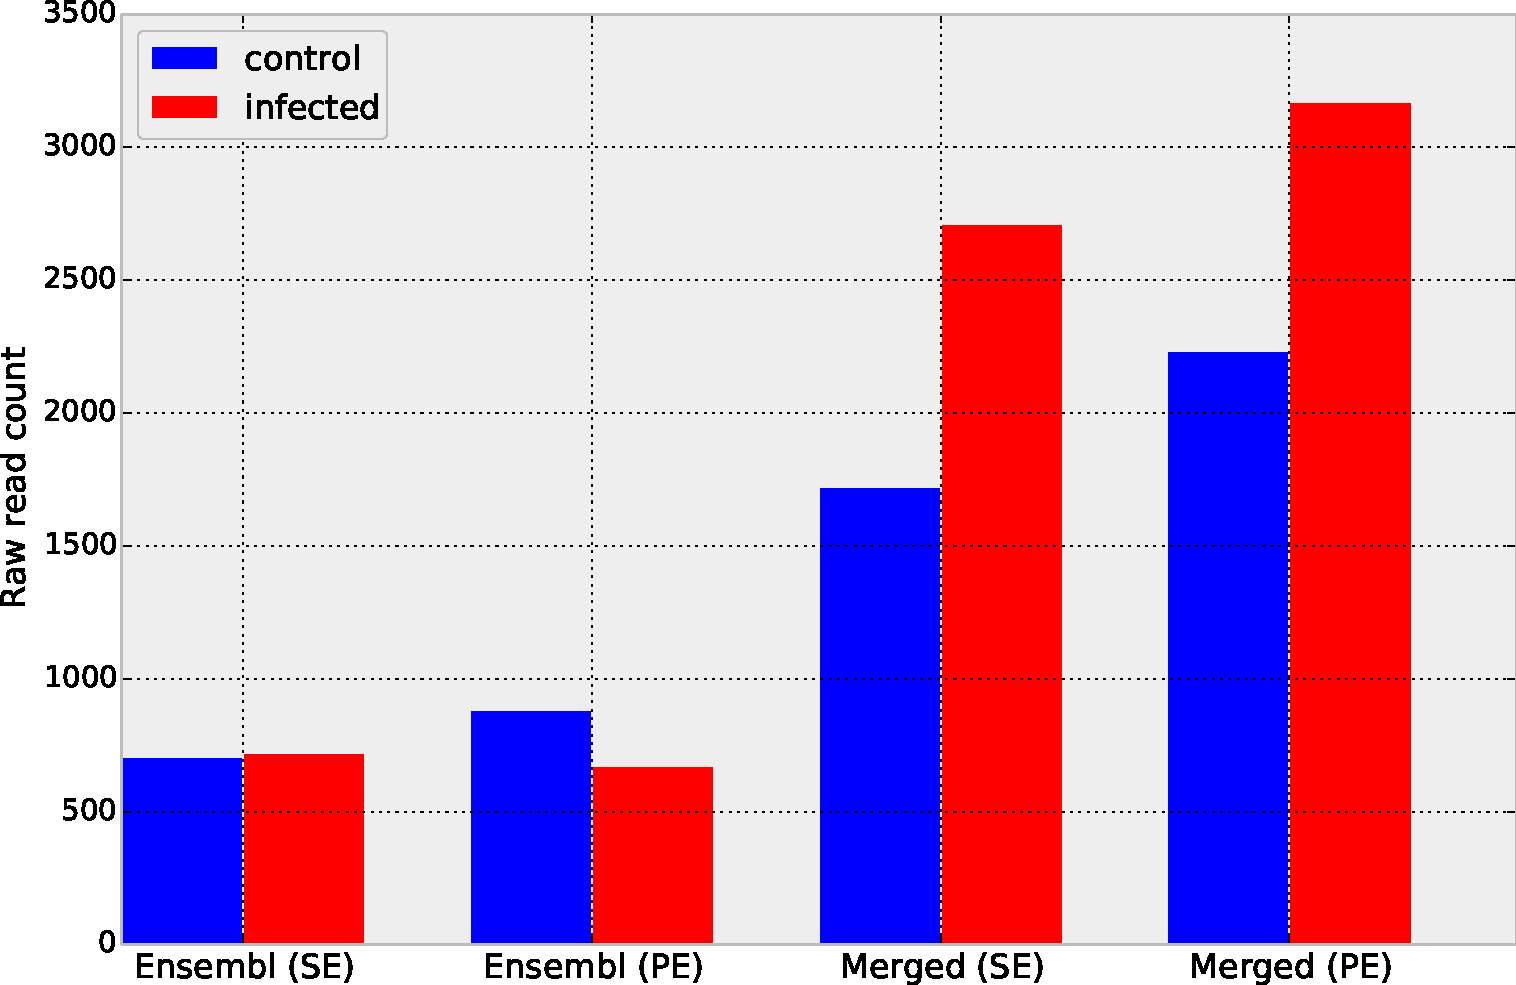
\includegraphics[width=6in]{idh3a-raw-reads-bar.pdf}
    \end{center}
    \caption{
        \textbf{Read counts of {\em IDH3A} gene.} SE=single-end, PE=paired-end
    }
    \label{idh3a_count}
\end{figure}

We next examined the gene size distribution across all four
gene model sets used (Figure~\ref{gene_length}).  Both the
Cufflinks {\em ab initio} gene models and the Gimme merged
gene models are significantly longer than the Ensembl and
assembly-based gene models, suggesting that they are more
complete.

% \pagestyle{empty}
% \begin{landscape}
\begin{figure}[!ht]
    \begin{center}
        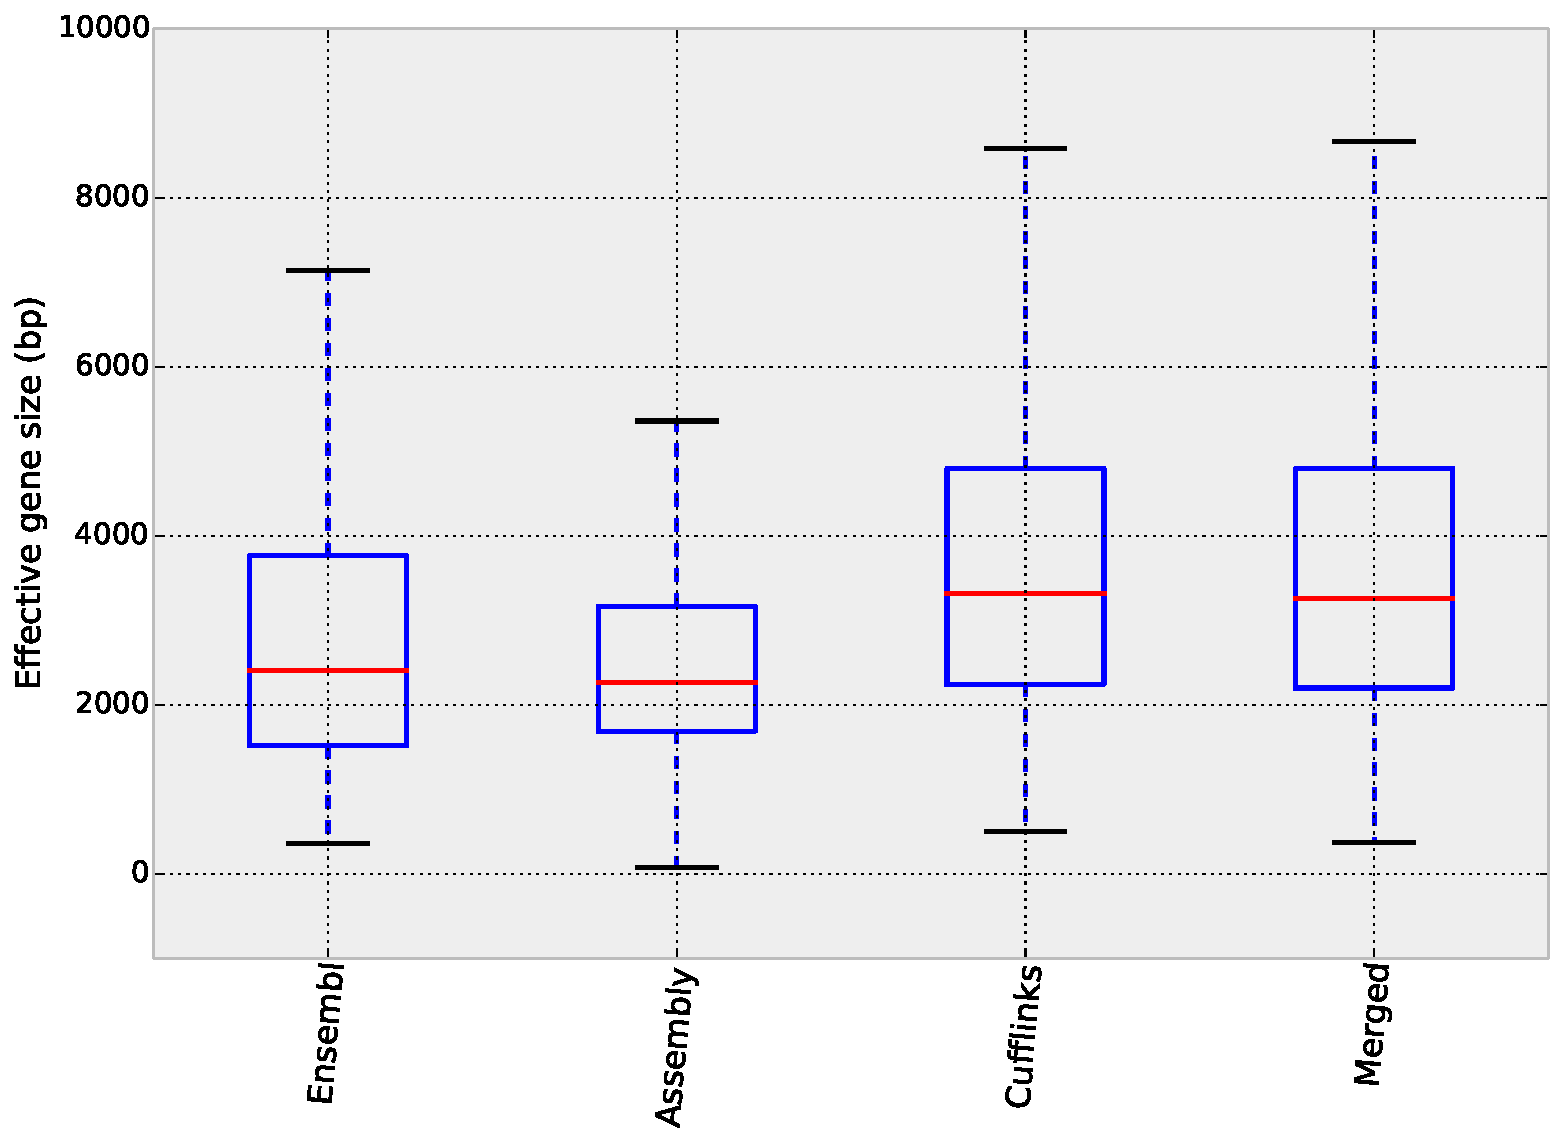
\includegraphics[width=6in]{gene_length.pdf}
    \end{center}
    \caption{
        \textbf{Gene sizes distribution.}
        Distribution of the same set of genes from different models are plotted.
        Sizes of genes in Ensembl models are slightly shorter than those from
        combined models. This is due partly to the fact that some genes may not
        contain UTRs.
        The sizes of genes from \textit{de novo} assembly are significantly smaller
        than other models indicating that transcripts are incomplete or fragmented.
    }
    \label{gene_length}
\end{figure}
% \end{landscape}
% \pagestyle{plain}

Finally, we examined the read counts and length-normalized
read counts for control and infected mRNAseq samples
(Figure~\ref{read_count}). In all cases, both the read
counts and length-normalized read counts were significantly
higher for the Gimme gene models.

% \pagestyle{empty}
% \begin{landscape}
\begin{figure}[!ht]
    \begin{center}
        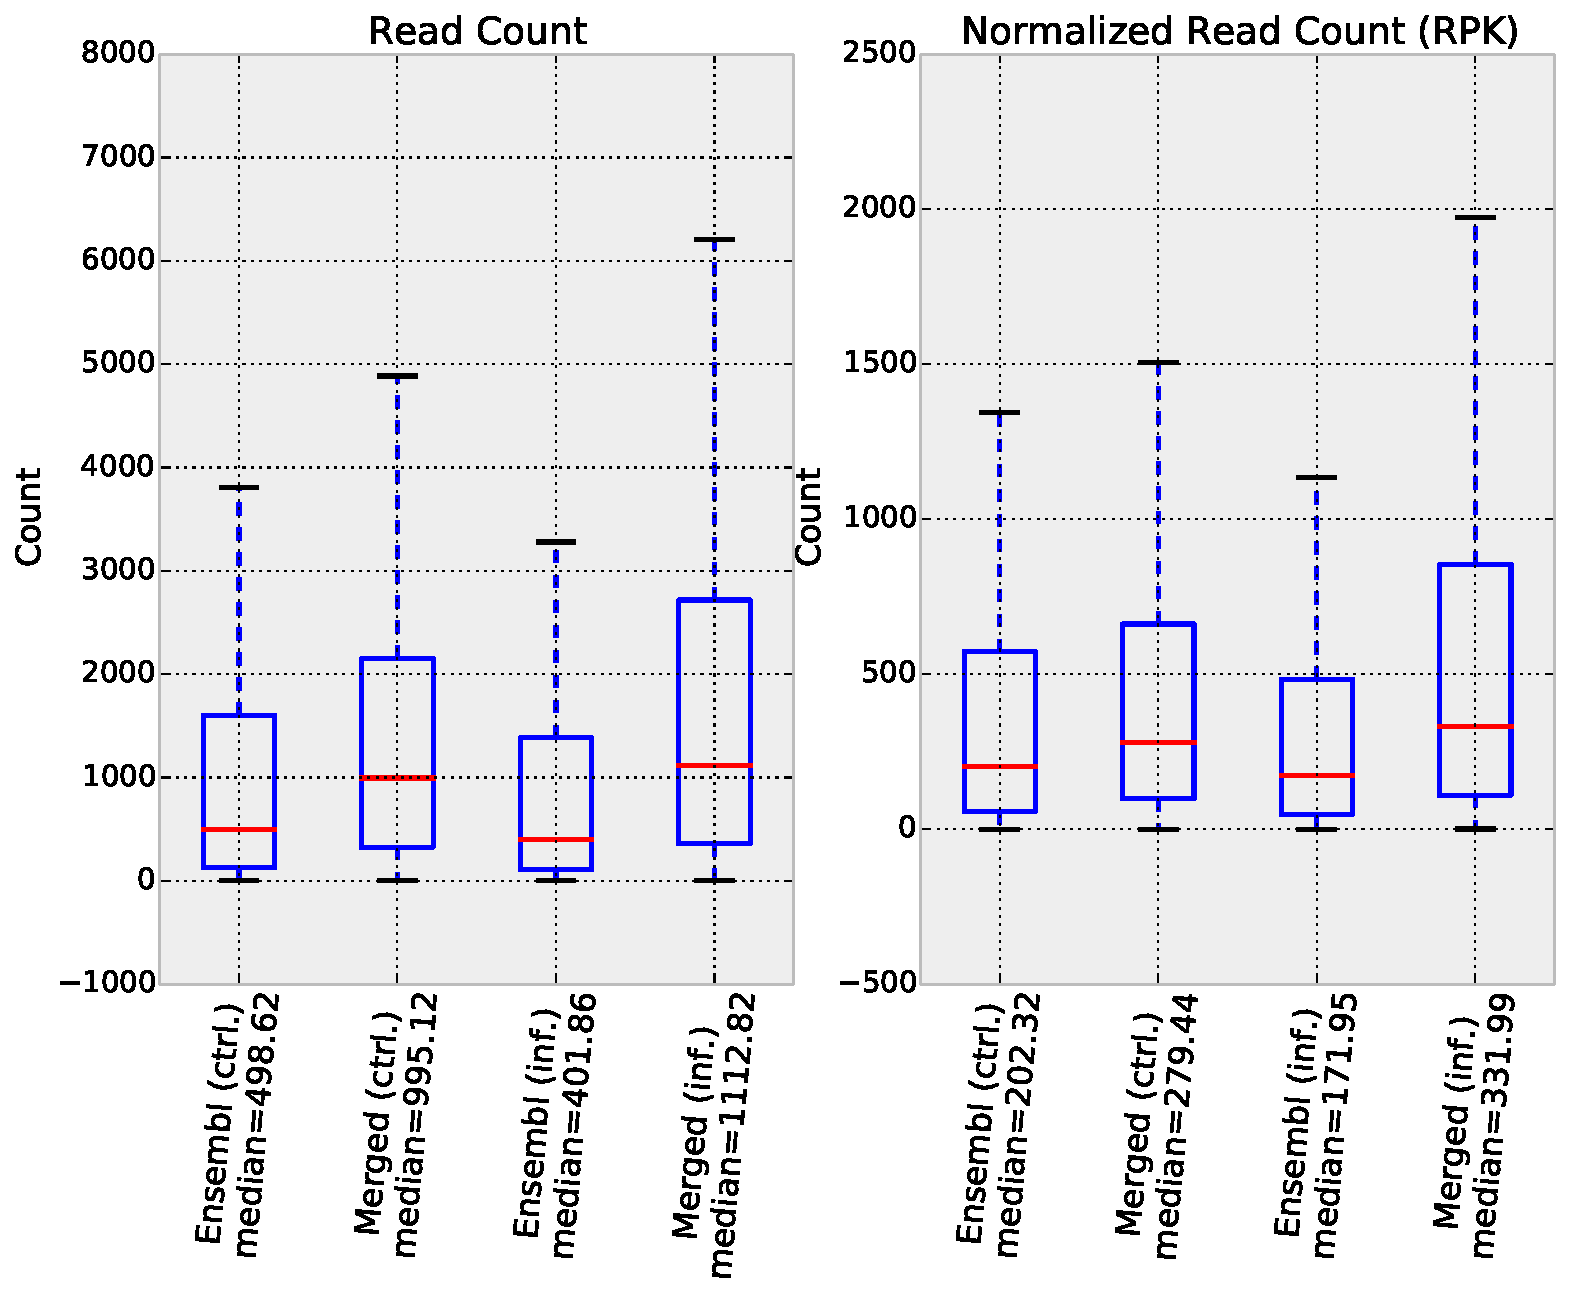
\includegraphics[width=6.5in]{read_count.pdf}
    \end{center}
    \caption{
        \textbf{Read counts comparisons.}
        In the same condition, read counts from Gimme models are significantly
        higher than those from Ensembl gene models.  Read counts are more
        similar after normalization by gene lengths.  Read counts were
        normalized by effective gene sizes using this formula: $1000 \times
        \frac{count}{length} = Read Per Kilobase (RPK)$.
    }
    \label{read_count}
\end{figure}
% \end{landscape}
% \pagestyle{plain}

To illustrate the effect of gene models variation on gene
expression estimates, comparisons of effective gene sizes
from all gene models and read counts from Ensembl and merged
models are shown in Figure~\ref{gene_length}
and~\ref{read_count}.  Effective gene sizes of 1,563
differential-expressed gene vary greatly among gene models
(Figure~\ref{gene_length}). The effective gene size is the
average of sizes of all transcripts from the same gene.  The
median of effective gene sizes of Ensembl models is 2413 bp
(IQR 2250 bp); whereas those of Cufflinks and merged models
are much higher (3320 bp (IQR 2550 bp) and 3270 bp (IQR 2595
bp) respectively).  This is expected because Cufflinks and
combined models are supposed to include UTRs.  On the other
hand, the median of the effective gene sizes of gene models
from {\em de novo} assembly is close to that of Ensembl
models; however, the IQR is much smaller (median = 2273 bp,
IQR = 1474 bp) suggesting that transcripts from \textit{de
novo} assembly are incomplete compared to Ensembl models.
The difference in gene sizes between Ensembl and combined
models results in a substantial deviation of read counts as
shown in Figure~\ref{read_count}.  Medians of read counts
from the same condition were significantly different between
Ensembl and combined models.  After normalization by gene
sizes, the difference were diminished suggesting that the
deviation of read counts is partly due to the size of the
gene models. 

\subsection{A majority of differential-expressed genes are
not annotated in KEGG pathway}

We next used the Kyoto Encyclopedia of Gene and Genomes
(KEGG) to annotate the differentially-expressed genes with
putative function and identify enriched pathways using
GOSeq~\cite{young2010method}.  Because there are only a
small number of species-specific chicken annotations in the
KEGG database, we also used homology search against human
Ensembl proteins (Release 74) to transfer gene annotations
from human genes to our chicken gene models.

Transferring gene annotations from human to chicken did not
result in a large increase in the number of genes that were
annotated, but the number of genes with pathway annotations
did increase.  In Figure~\ref{num_kegg}, we show the effect
of this transfer on the pathway annotations for different
gene model sets.
% LP the results below changed significantly. I might have
% done something wrong before.
For the merged data set, $\sim$27\% of DE gene models had
species-specific KEGG annotations, while approximately 36\%
had human KEGG annotations.

\begin{figure}[!ht]
    \begin{center}
        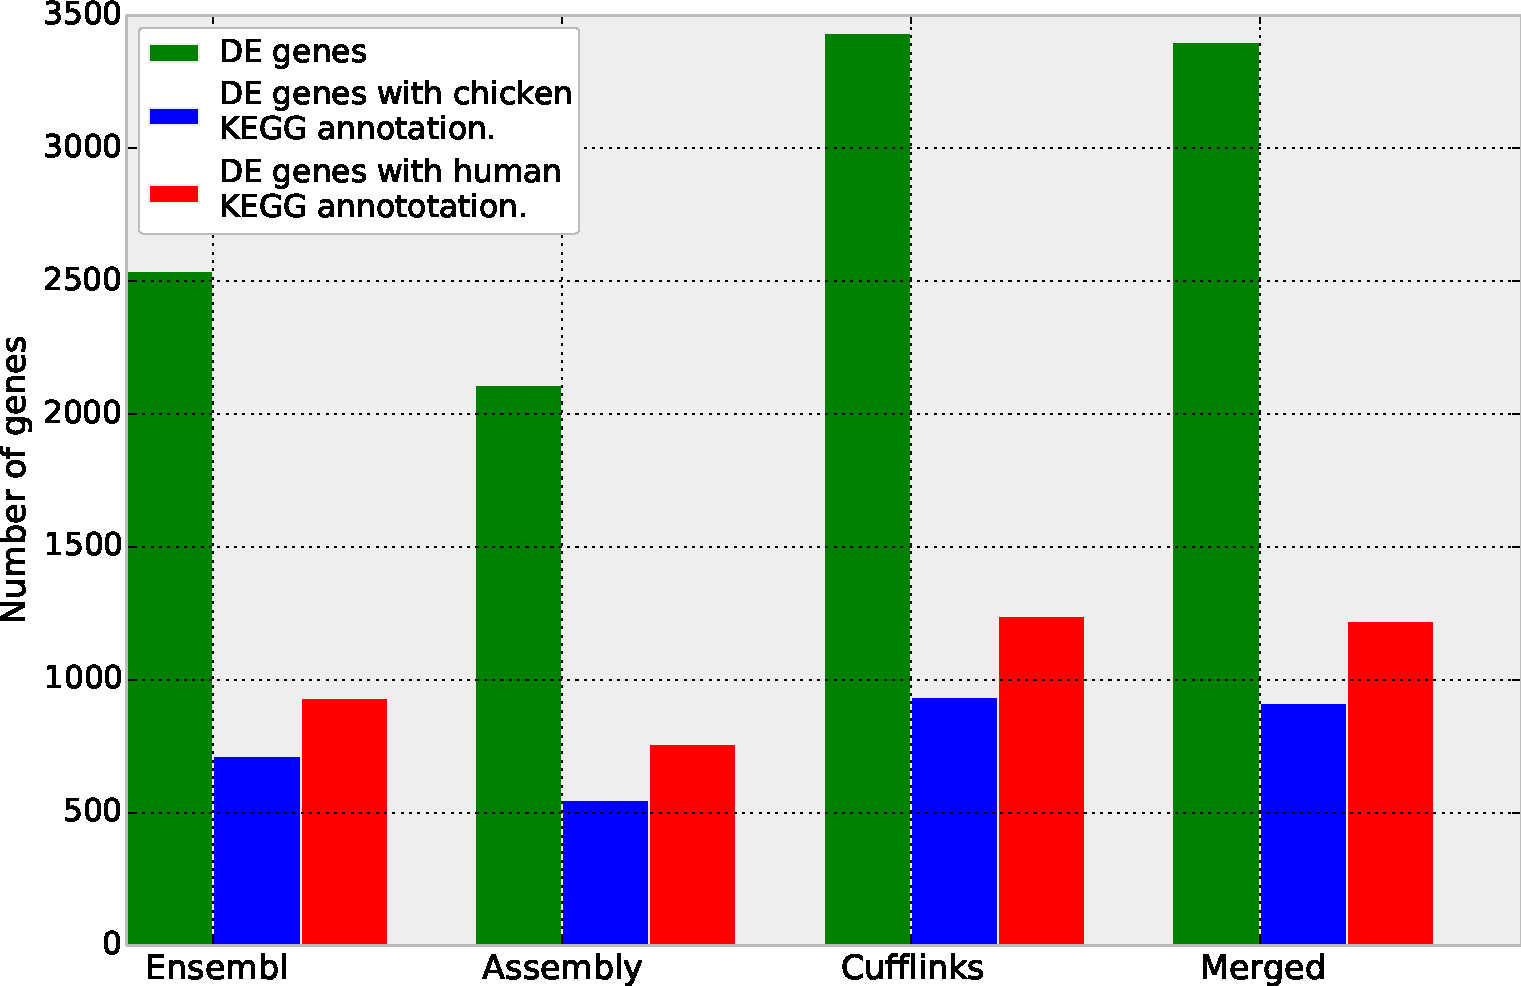
\includegraphics[width=6in]{gallus-hsa-num-kegg-genes-bar.pdf}
    \end{center}
    \caption{
        \textbf{DE genes with chicken and human KEGG annotations.}
    }
    \label{num_kegg}
\end{figure}

Unsurprisingly, transferring gene annotations also led to a
dramatic difference in the KEGG pathways predicted to be
enriched between the two conditions.
Figure~\ref{gimme_hs_ga} shows the enriched KEGG pathways in
the merged gene models with first, only chicken annotation
and second, with transferred human annotations.  A total of
26 pathways were predicted to be enriched in one or both of
the annotation sets, with 6 in common, 9 unique to the
species-specific annotations, and 11 unique to the human
annotation set.  A majority of the chicken-specific
annotations were immune system annotations, reflecting the
extensive work done on chicken
immunity~\cite{burt2005chicken}.

\subsection{Pathway predictions vary widely between gene
model sets}

To compare the pathway predictions using chicken+human
annotations, we calculated the Spearman rank correlation
coefficient for all possible pair-wise comparisons.  The results,
shown in Table~\ref{tab:spearmanr}, show that the correlations
are very poor.  The weakest correlation is between the pathway
predictions for the Ensembl gene model set and the merged gene
model set.

\begin{table}[!ht]
\caption{
\textbf{Spearman Rank Correlation}}
\begin{center}
\begin{tabular}{ccccc}
\hline
& Assembly & Ensembl & Cufflinks & Merged \\
\hline
Assembly & 1.0 & 0.39 & 0.45 & 0.50 \\
Ensembl & & 1.0 & 0.48 & 0.36 \\
Cufflinks & & & 1.0 & 0.76 \\
Merged & & & & 1.0 \\
\hline
\end{tabular}
\end{center}
%\begin{flushleft}
%    (-) down-regulated, (+) up-regulated
%\end{flushleft}
\label{tab:spearmanr}
\end{table}

% @CTB: what is the goal of these last two sentences? An
% example of how they are different.
Five pathways are predicted to be enriched only when using
the Ensembl gene models (Figure~\ref{KEGG_all}), including
the antigen processing and presentation pathway, which is
important for immune responses.  In addition, the T cell
receptor signaling pathway is predicted to be enriched in
all of the gene model sets excepting only the Ensembl
models.

The correlation coefficient between enriched pathways
predicted from Ensembl gene models and Cufflinks gene models
is rather high, which may be because the Ensembl models were
integrated with RNA-Seq data to construct the Cufflinks
models.  The integration is done based on the criteria that
incomplete transcripts or transcripts without novel introns
compared to the Ensembl models are discarded and UTRs from
RNA-Seq data are used to extend Ensembl UTRs
~\cite{roberts2011identification}.  Therefore, Cufflinks
models are a superset of the Ensembl models and should
contain all pathways from Ensembl models.  However, eighteen
pathways are unique to Cufflinks and seven pathways are
unique to Ensembl; this may be due to a difference in the
read mapping percentage.
% @CTB: or just statistics, right?  More genes, different
% cutoffs...

Finally, the correlation between enriched pathways predicted
using the Cufflinks-based differential expression and the
Gimme-based differential expression is the highest.
Although twelve enriched pathways are unique to Cufflinks,
and four pathways are unique to the merged models, the
correlation coefficient is high because the common pathways
have similar significance scores.  Twenty nine enriched
pathways are different between the merged models and Ensembl
and this results in a slightly lower correlation coefficient
than that between the combined models and Cufflinks.
Table~\ref{tab:combined_unique} shows common and unique
enriched pathways from Ensembl and combined models.  A
majority of unique enriched pathways from Ensembl are
involved in metabolism and cellular activities.
% @Jerry: the following paragrah is not an explanation
In contrast, unique pathways from combined models are
involved in immune response and cancer, which we would
expect to be perturbed by MDV infection.

\begin{table}[!ht]
\caption{
\textbf{Pathways from Ensembl and merged gene models}}
\begin{center}
\begin{tabular}{ccc}
\hline
pathway ID & Term & Adjusted p-value \\
\hline
& Pathways in Ensembl only & \\
\hline
00980 & Metabolism of xenobiotics by cytochrome P450 & 2.3e-06 \\
00480 & Glutathione metabolism & 1.9e-05 \\
00982 & Drug metabolism - cytochrome P450 & 9.5e-04 \\
04142 & Lysosome & 1.1e-03 \\
04010 & MAPK signaling pathway & 3.0e-03 \\
00400 & Phenylalanine, tyrosine and tryptophan biosynthesis & 3.4e-03 \\
00500 & Starch and sucrose metabolism & 4.9e-03 \\
00983 & Drug metabolism - other enzymes & 5.5e-03 \\
00360 & Phenylalanine metabolism & 6.3e-03 \\
\hline
& Common pathways & \\
\hline
04060 & Cytokine-cytokine receptor interaction & 5.8e-15 \\
04145 & Phagosome & 4.7e-07 \\
01100 & Metabolic pathways & 1.1e-06 \\
04620 & Toll-like receptor signaling pathway & 4.8e-05 \\
04623 & Cytosolic DNA-sensing pathway & 1.2e-04 \\
04210 & Apoptosis & 1.8e-04 \\
04630 & Jak-STAT signaling pathway & 2.1e-04 \\
04672 & Intestinal immune network for IgA production & 2.4e-04 \\
04622 & RIG-I-like receptor signaling pathway & 3.6e-04 \\
04621 & NOD-like receptor signaling pathway & 1.4e-03 \\
04650 & Natural killer cell mediated cytotoxicity & 2.0e-03 \\
\hline
& Pathways in merged models only & \\
\hline
04514 & Cell adhesion molecules (CAMs) & 1.8e-04 \\
04141 & Protein processing in endoplasmic reticulum & 10.0e-04 \\
04510 & Focal adhesion & 2.3e-03 \\
04512 & ECM-receptor interaction & 3.3e-03 \\
\hline
\end{tabular}
\end{center}
\begin{flushleft}
\end{flushleft}
\label{tab:combined_unique}
\end{table}

% @CTB: this text belongs in either introduction or
% discussion, not in results!
For non-model organisms without high-coverage functional
pathway annotation or gene ontology (GO), an alternative
method for functional analysis is to use pathway annotations
of closely related or well-studied model organisms such as
mouse and human.  This approach could increase
sensitivity of pathway analysis; however, it will not
include species-specific genes and pathways.  For instance,
in this study, some pathways involved in chicken immune
responses including natural killer cell mediated
cytotoxicity, intestinal immune network for IgA production,
and focal adhesion were not enriched in human annotation
with merged models (Figure~\ref{gimme_hs_ga}).

\begin{figure}[!ht]
    \begin{center}
        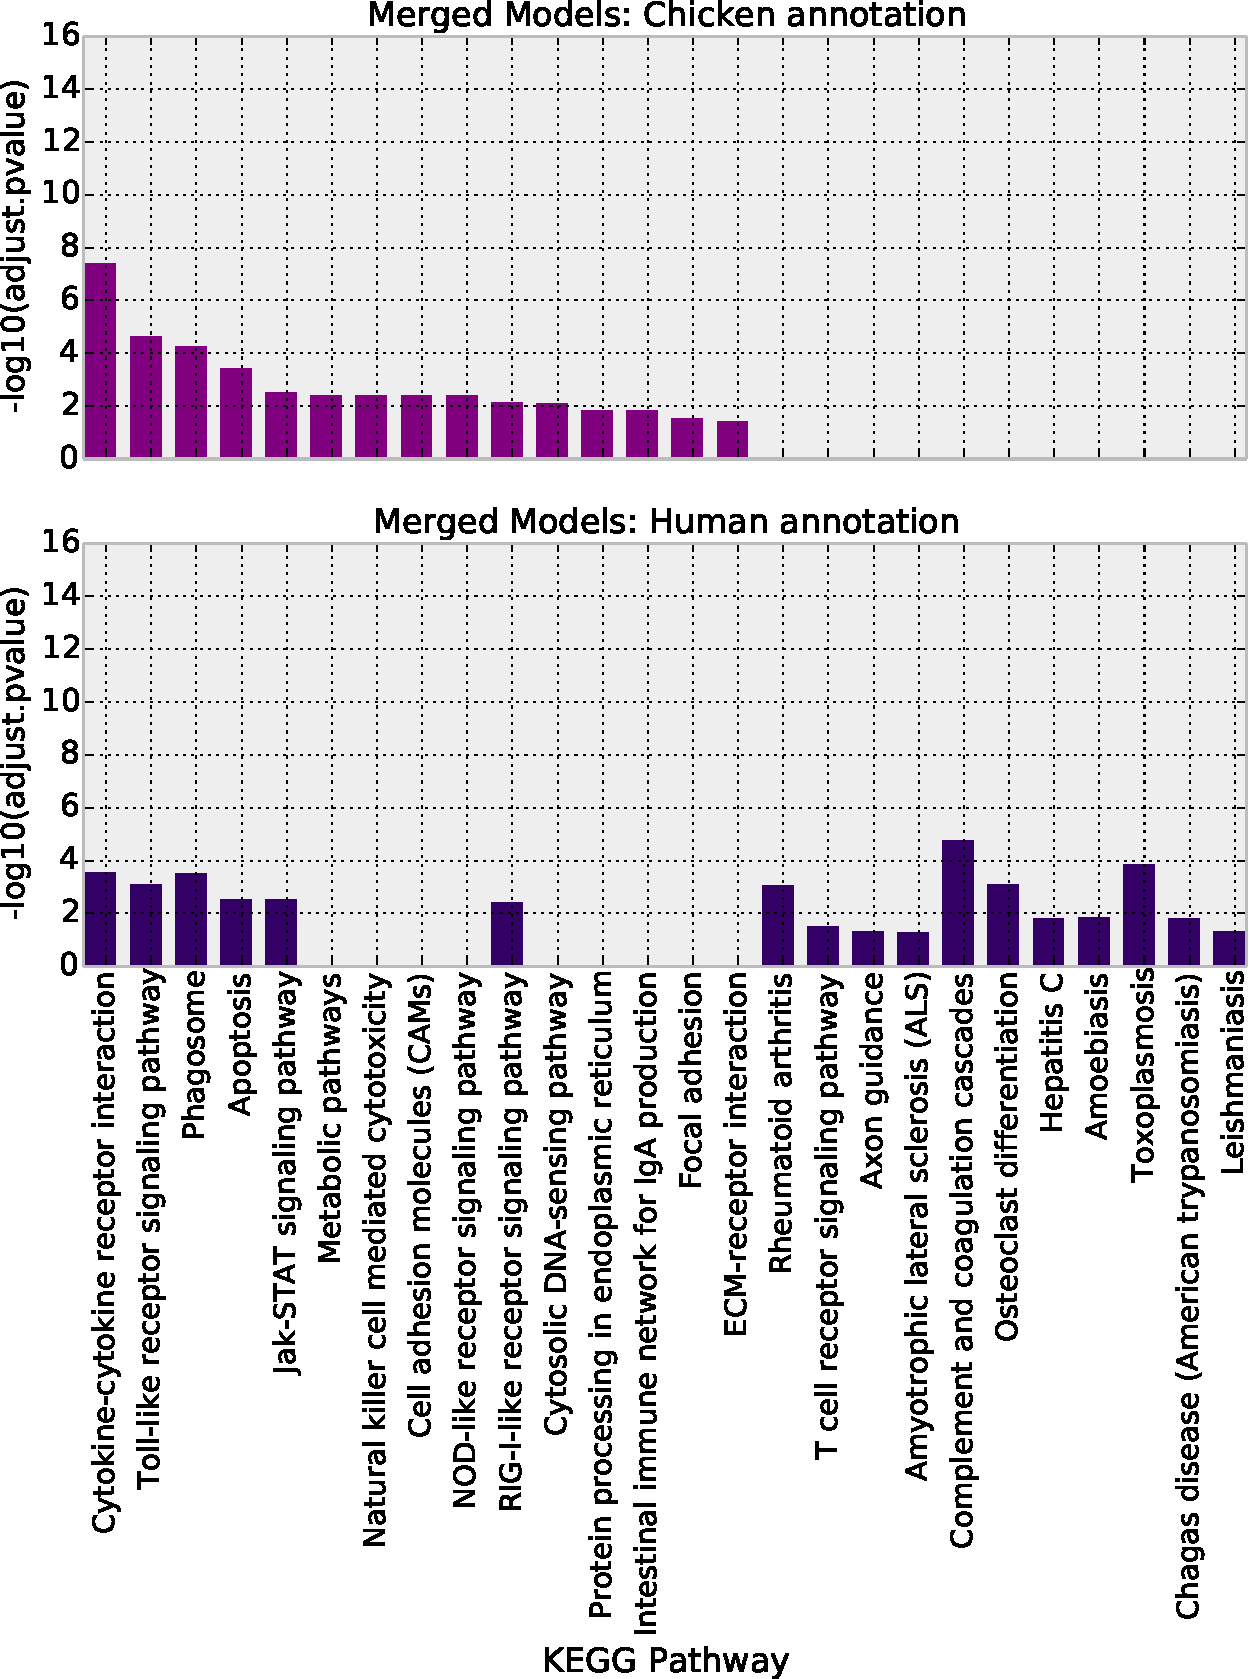
\includegraphics[width=6in]{gimme-hsa-gga-kegg-pvalue-bar.pdf}
    \end{center}
    \caption{
        \textbf{Enriched KEGG Pathways from merged models with
        chicken and human annotation}
    }
    \label{gimme_hs_ga}
\end{figure}

To overcome this problem, we propose to use a custom pathway
annotation built from a combination of annotations from the
organism and related species.  To validate our method, we
built a custom annotation by assigning human annotations to
chicken genes with no pathway annotations and used the
custom annotation for pahtway analysis.  The results (shown
at the bottom graph of Figure~\ref{KEGG_all}) include some
significantly enriched pathways involved in immune responses
such as complement and coagulation cascades, T cells
receptor pathway, and chemokines signaling pathway. Almost
all enriched pathways from either Cufflinks or Ensembl
models are also included.  Besides the top three most
significant pathways, pathways from custom annotations,
Cufflinks and Ensembl have only slightly different
significance scores.  This indicates that custom annotation
can help increase the sensitivity of pathway analysis,
especially in semi-model organisms.  However, results have
to be interpreted with great care due to biological
differences between organisms.

\begin{figure}[!ht]
    \begin{center}
        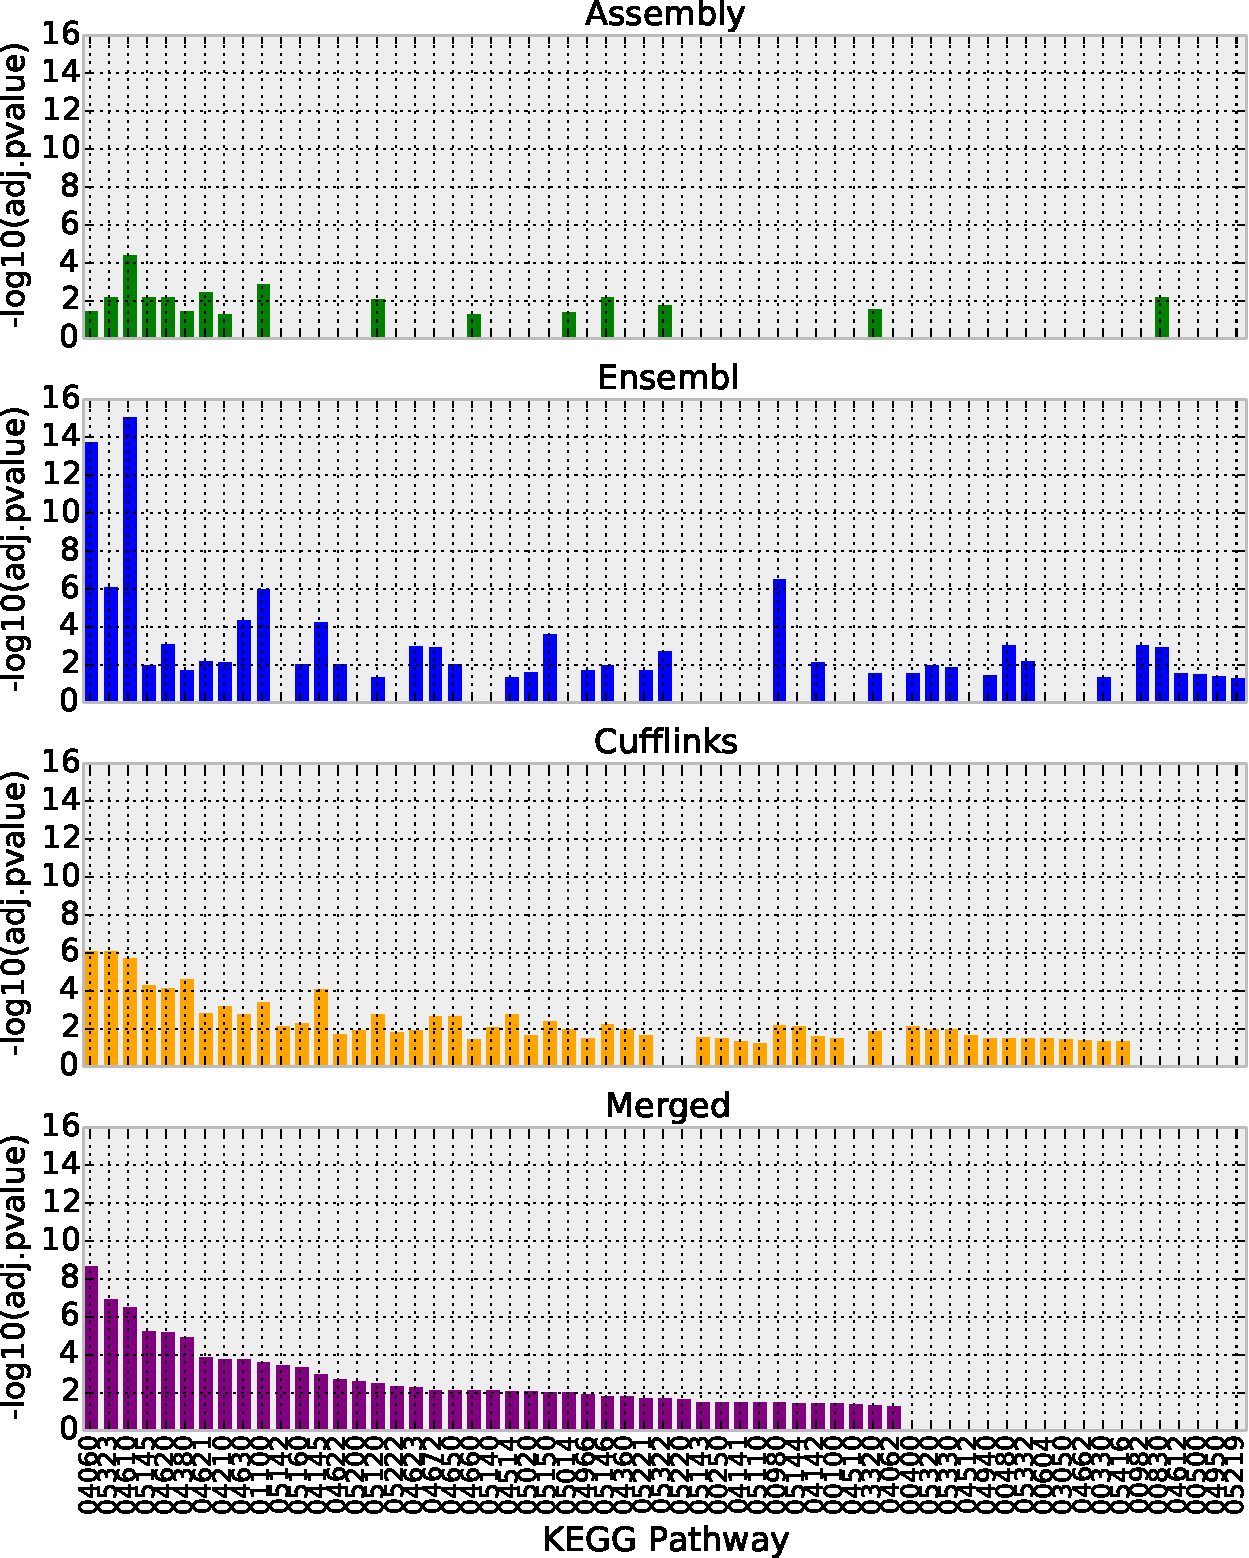
\includegraphics[width=6in]{gallus-kegg-pvalue-bar.pdf}
    \end{center}
    \caption{
        \textbf{Enriched KEGG Pathways from different gene models}
    }
    \label{KEGG_all}
\end{figure}

\section{Discussion}

\subsection{Variation in gene model sets greatly affects expression estimates}

Methods for differential gene expression analysis typically
estimate gene expression from the number of reads mapped to
each gene model.  Reads that do not map to gene models, such
as reads belonging to unannotated UTRs or exons, are
generally excluded.  This exclusion leads to insensitivity
in estimates of expression, and can be particularly
problematic when genes have long UTRs and uenven read
coverage.

Here, we show that using the same parameters for mapping and
differential exprssion analysis with several different gene
model sets results in large differences in both read mapping
and the prediction of differentially expressed (DE) genes.
While some differences are expected, we found that the
differences were surprisingly large: for most of the
comparisons, the DE genes disjoint between the two gene
model sets were larger in number than the DE genes shared
between the two gene model sets.

These differences are due to differences in the number of
reads mapping to the gene models.  Unsurprisingly, many more
reads map to the gene model data sets constructed from the
mRNAseq data -- between 15\% and 20\%
(Table~\ref{tab:mapped-reads}).  This results in many more
reads mapping to each gene model (Figure~\ref{gene_length}a)
and significantly higher RPKM estimates for each mRNAseq
data set (Figure~\ref{gene_length}b).

\subsection{Conclusion}

As the use of RNA-Seq to study semi- and non-model organisms
has vastly increased recently, one objective of this study
is to demonstrate the potential problem of transcriptome
study in organisms that lack high quality genome, gene
models and functional pathway annotation.  Gene models
derived from {\em de novo} assembly are usually the only
choice for those organisms; however, the results are
relatively poor compared to others.  Custom gene models
built from Cufflinks (integrated with Ensembl) helped
increase sensitivity of pathway analysis and should be used
if a reference genome is available and {\em de novo}
assembly is not feasible.  However, the method is reliant on
a quality of a genome sequence and subject to read-mapping
biases.  Combined gene models, although appearing to have
lower sensitivity compared to those from Cufflinks and
Ensembl, still recover most of the pathways with high
significance scores.  The advantage of using combined gene
models is it allows the integration of gene models from {\em
de novo} assembly, which are not affected by read-mapping
biases.  Results from our study show that they significantly
increase sensitivity of genes and isoforms
detection.  Depending on available resources and the
objective of the study, we suggest that appropriate gene
models should be carefully chosen to maximize the quality of
the analysis.  Moreover, using functional pathway annotation
from a related species is always necessary for those
organisms, but it will not include species-specific genes
and pathways. The problem is compounded when only gene
models from {\em de novo} assembly are available. Therefore,
biologists studying non-model organisms need to be aware of
these limitations when interpreting the results from
transcriptome analysis.


% You may title this section "Methods" or "Models". 
% "Models" is not a valid title for PLoS ONE authors. However, PLoS ONE
% authors may use "Analysis" 
\section{Materials and Methods}

\subsection{Sequences and quality trimming}

mRNAs were extracted from spleens of control and infected
line 7 chickens (14 dpi).  Sequence libraries were prepared
by standard Illumina unstranded single- and paired-end
protocols.  Library size of the paired-end datasets is
approximately 175 bp.  Read lengths are 75 bp in both
single- and paired-end libraries.  Reads were quality
trimmed by condetri 2.1~\cite{smeds2011condetri} with
quality score cutoff of 30.  The first 10 bases were removed
due to a non-uniform distribution of nucleotides.

\subsection{Custom gene models construction}

Reads were mapped to chicken genome (galGal4) by TopHat
2.0.9~\cite{Trapnell:2009dp} and gene models were
constructed with Ensembl models release 73 as a reference by
Cufflinks 2.1.1~\cite{Trapnell:2010kd}.  Velvet
1.2.03~\cite{Zerbino:2008vu} and Oases
0.2.06~\cite{Schulz:2012je} were used to assemble reads with
hash lengths ranging from $21-31$.  Transcripts from all
hash lengths were then reassembled with OasesM.  Combined
gene models were constructed by Gimme~\cite{gimme:Online},
which combined Cufflinks models and alignments of \textit{de
novo} transcripts to the genome.  Transcripts were mapped to
the genome using BLAT~\cite{Kent:2002tv} and for each
transcript, only an alignment with the best mapping score
was used.


\subsection{Differential gene expression and gene ontology}

Quality filtered reads were mapped to transcripts from all
gene models without poly-A tail added by Bowtie
1.0~\cite{langmead2009ultrafast}.  Estimated gene expression
and differential expression analysis was performed by RSEM
1.2.7~\cite{li2011rsem} and EBseq~\cite{leng2013ebseq}
respectively.  DE genes were annotated by homologous
sequences in chicken and human proteins from Ensembl release
73 and 74 respectively.  GOSeq 1.14.0~\cite{young2010method}
was used to perform enrichment analysis using KEGG
annotations from org.Gg.eg.db~\cite{Gg} and
org.Hs.eg.db~\cite{Hs}.  Human KEGG annotations were added
to all DE genes to create combined KEGG pathways.

\subsection{Pipeline and scripts}

The pipeline and scripts used in this study is available at

\texttt{https://github.com/likit/RNASeq-methods-comparison}
